\documentclass[12pt,aspectratio=169]{beamer}

% ====================================================
% ====================================================
% USEPACKAGES AND IMPORTS
% ====================================================
% ====================================================

\usepackage[T1]{fontenc}
\usepackage[utf8]{inputenc}
\usepackage[english]{babel}

% tables
\usepackage{tabularx}
\usepackage{colortbl}
\usepackage{multirow}
\usepackage{makecell}

% tikz and colors
\usepackage{tikz}
\usepackage{xcolor}
\usepackage{pgfplots}
\usepackage{pgfplotstable}
\usepackage{tikzsymbols}

\usetikzlibrary{calc}
\usetikzlibrary{trees}
\usetikzlibrary{patterns}
\usetikzlibrary{shadings}
\usetikzlibrary{positioning}
\usetikzlibrary{intersections}
\usepgfplotslibrary{patchplots}
\usepgfplotslibrary{fillbetween}
\usetikzlibrary{decorations.pathreplacing}

\usetikzlibrary{arrows}
\usetikzlibrary{arrows.meta}

\usetikzlibrary{shapes}
\usetikzlibrary{shapes.arrows}
\usetikzlibrary{shapes.callouts}
\usetikzlibrary{shapes.symbols}
\usetikzlibrary{shapes.geometric}

% boxes
\usepackage[many]{tcolorbox}

% math packages and fonts
\usepackage{bm}
\usepackage{ccfonts}
\usepackage{eulervm}
\usepackage{amsmath}
\usepackage{amsfonts}
\usepackage{amssymb}
\usepackage{amsthm}
\usepackage{mathtools}
\usepackage{nicefrac}
\usepackage{slashed}
\usepackage{bbold}
\usepackage{array}
\usepackage{cancel}

% algorithms and listings
\usepackage[ruled,vlined,linesnumbered]{algorithm2e}
\usepackage{listings}
\usepackage{setspace}

\tcbuselibrary{listings}
\tcbuselibrary{breakable}
\tcbuselibrary{skins}

% misc
\usepackage{soul}
\usepackage{pifont}
\usepackage{skull}
\usepackage{multicol}
\usepackage{animate}
\usepackage{hyperref}
\usepackage{wasysym}
\usepackage[absolute,overlay]{textpos}
\usepackage[hang,flushmargin]{footmisc}

% ====================================================
% ====================================================
% LAYOUT AND THEME
% ====================================================
% ====================================================

\usetheme{Copenhagen}

% color definitions
\definecolor{myblue1}{RGB}{35,119,189}
\definecolor{myblue2}{RGB}{95,179,238}
\definecolor{myblue3}{RGB}{129,168,207}
\definecolor{myblue4}{RGB}{26,89,142}

\definecolor{myred1}{RGB}{247,12,12}

% set theme colors
\setbeamercolor*{structure}{fg=myblue1,bg=blue}
\setbeamercolor*{palette primary}{use=structure,fg=white,bg=structure.fg}
\setbeamercolor*{palette secondary}{use=structure,fg=white,bg=structure.fg!75!black}
\setbeamercolor*{palette tertiary}{use=structure,fg=white,bg=structure.fg!50!black}
\setbeamercolor*{palette quaternary}{fg=black,bg=white}

\setbeamertemplate{itemize item}[circle]
\setbeamertemplate{itemize subitem}[circle]
\setbeamertemplate{itemize subsubitem}[circle]

\setbeamertemplate{enumerate item}[circle]
\setbeamertemplate{enumerate subitem}[circle]
\setbeamertemplate{enumerate subsubitem}[circle]

\setbeamercolor{itemize item}{fg=myblue1}
\setbeamercolor{itemize subitem}{fg=myblue1}
\setbeamercolor{itemize subsubitem}{fg=myblue1}

\setbeamertemplate{section in toc}[circle]
\setbeamertemplate{subsection in toc}[circle]
\setbeamerfont{subsection in toc}{size=\scriptsize}

\setbeamercolor{frametitle continuation}{fg=black}

% title graphic -- sap logo and dhbw logo
\titlegraphic{
\includegraphics[scale=0.1]{../03_img/logo_sap}\hspace*{4.75cm}~%
   	
\includegraphics[scale=0.05]{../03_img/logo_dhbw}
}

\makeatletter
% frame title
\defbeamertemplate*{frametitle}{mydefault}[1][left]
{
  	\ifbeamercolorempty[bg]{frametitle}{}{\nointerlineskip}%
  	\nointerlineskip%
 	\@tempdima=\textwidth%
  	\advance\@tempdima by\beamer@leftmargin%
  	\advance\@tempdima by\beamer@rightmargin%
  	\begin{tcolorbox}[
  		enhanced,
  		outer arc=0pt,
  		arc=0pt,
  		boxrule=0pt,
  		top=0pt,
  		bottom=0pt,
  		enlarge left by=-\beamer@leftmargin,
  		enlarge right by=-\beamer@rightmargin,
  		width=\paperwidth,
  		nobeforeafter,
  		interior style={
    			left color=myblue2,
    			right color=white
    		},
  		shadow={0mm}{-0.4mm}{0mm}{black!60,opacity=0.6},    
  		shadow={0mm}{-0.8mm}{0mm}{black!40,opacity=0.4},    
  	]
    	\usebeamerfont{frametitle}%
    	\vbox{}\vskip-1ex%
    	\if@tempswa\else\csname beamer@fte#1\endcsname\fi%
    	\insertframetitle\par%
    	{%
      		\ifx\insertframesubtitle\@empty%
      		\else%
      		{\usebeamerfont{framesubtitle}\usebeamercolor[fg]{black}\insertframesubtitle\strut\par}%
      		\fi
    	}%
    	\vskip-1ex%
    	\if@tempswa\else\vskip-.3cm\fi
  	\end{tcolorbox}%
}

% footline of a frame
\defbeamertemplate*{footline}{mysplit theme}
{%
  	\leavevmode%
  	\hbox{
		\begin{beamercolorbox}[
			wd=.5\paperwidth,ht=2.5ex,dp=1.125ex,leftskip=.3cm plus1fill,rightskip=.3cm
		]{author in head/foot}%
    			\usebeamerfont{author in head/foot}\insertshortauthor\ (\insertinstitute), \insertdate
  		\end{beamercolorbox}%
  		\begin{beamercolorbox}[
			wd=.5\paperwidth,ht=2.5ex,dp=1.125ex,leftskip=.3cm,rightskip=.3cm plus1fil
		]{title in head/foot}%
    			\usebeamerfont{title in head/foot}\insertshorttitle\hfill
    			\insertprefix-\insertframenumber/\inserttotalframenumber\hspace*{0.5em}
  		\end{beamercolorbox}}%
  	\vskip0pt%
}
\makeatother

% ====================================================
% ====================================================
% COMMANDS AND GENERAL DEFINITIONS
% ====================================================
% ====================================================

% page number prefix
\newcommand\insertprefix{}  % empty by default
\newcommand\prefix[1]{\renewcommand\insertprefix{#1}}

% math definitions
% ====================================================
\DeclareMathOperator*{\argmax}{arg\,max}
\DeclareMathOperator*{\argmin}{arg\,min}
\newcommand*\diff{\mathop{}\!\mathrm{d}}

\newcommand*{\vertbar}{\rule[-1ex]{0.5pt}{2.5ex}}
\newcommand*{\horzbar}{\rule[.5ex]{2.5ex}{0.5pt}}

% commands
% ====================================================

% highlight commands
% --------------------------------------------------------------------------------------------------------
% highlight command
\newcommand{\highlight}[1]{\textcolor{myblue1}{\textbf{#1}}}
\newcommand{\highlighttt}[1]{\textcolor{myblue1}{\texttt{#1}}}
\newcommand{\Highlight}[1]{\textcolor{myred1}{\textbf{#1}}}

% blue color boxes (with frame/without frame/without fill)
\newtcolorbox{boxBlue}{colback=myblue1!10!white,colframe=myblue4}
\newtcolorbox{boxBlueNoFrame}{colback=myblue1!10!white,colframe=myblue1!10!white}
\newtcolorbox{boxBlueNoFill}{colback=white,colframe=myblue4}

% font commands
% --------------------------------------------------------------------------------------------------------
\newcommand{\linkstyle}[1]{\underline{\smash{\texttt{#1}}}} 		% style of hyperlinks

% tikz commands
% --------------------------------------------------------------------------------------------------------

% yellow sticky note
\newcommand{\bubble}[3]{
\begin{textblock}{100}(#1, #2)
      	\begin{tikzpicture}
		\node[rectangle,draw=yellow,very thick,fill=yellow!60,align=center] at (0,0) {#3};
	\end{tikzpicture}
\end{textblock}
}

\newcommand{\floattext}[3]{
\begin{textblock}{100}(#1, #2)
      	#3
\end{textblock}
}

\newcommand{\doublecircle}[2]{
	\draw[fill=white,draw=myblue1] (#1,#2) circle (2mm);
	\draw[fill=myblue1,draw=myblue1] (#1,#2) circle (1.5mm);
}

% slide modifiers
% --------------------------------------------------------------------------------------------------------
% mark slide as optional
\newcommand{\optional}{
	\begin{textblock}{100}(0.15,0.30)
      		
\includegraphics[scale=0.2]{../03_img/scream}
    	\end{textblock}
}

% mark slide as important
\newcommand{\important}{
	\begin{textblock}{100}(0.10,0.15)
      		
\includegraphics[scale=0.1]{../03_img/important}
    	\end{textblock}
}

% citation
% --------------------------------------------------------------------------------------------------------
% first argument in {book, online, article}
\newcommand{\literature}[5]{
	\setbeamertemplate{bibliography item}[#1]
	\bibitem{#2}
	\highlight{#3} \\
	\textcolor{darkgray}{\textit{#4}} \\
	\textcolor{black}{#5}
}
% cite content
\newcommand{\citeAuthor}[3]{\vfill\scriptsize\textcolor{lightgray}{#1 \cite{#2} #3}}

% slide architecture
% --------------------------------------------------------------------------------------------------------
% divide frame into two parts
\newcommand{\divideTwo}[4]{
	\begin{minipage}{#1\textwidth}
		#2
	\end{minipage}
	\hfill
	\begin{minipage}{#3\textwidth}
		#4
	\end{minipage}
}

% divide frame into two parts (start on top)
\newcommand{\divideTwoTop}[4]{
	\begin{minipage}[t]{#1\textwidth}
		#2
	\end{minipage}
	\hfill
	\begin{minipage}[t]{#3\textwidth}
		#4
	\end{minipage}
}

% special pages
% --------------------------------------------------------------------------------------------------------
% title page
\newcommand{\maketitlepage}{
	{
		\beamertemplatenavigationsymbolsempty
		\usebackgroundtemplate{%
			\tikz[overlay,remember picture] \node[opacity=0.2, at=(current page.center)] {
  				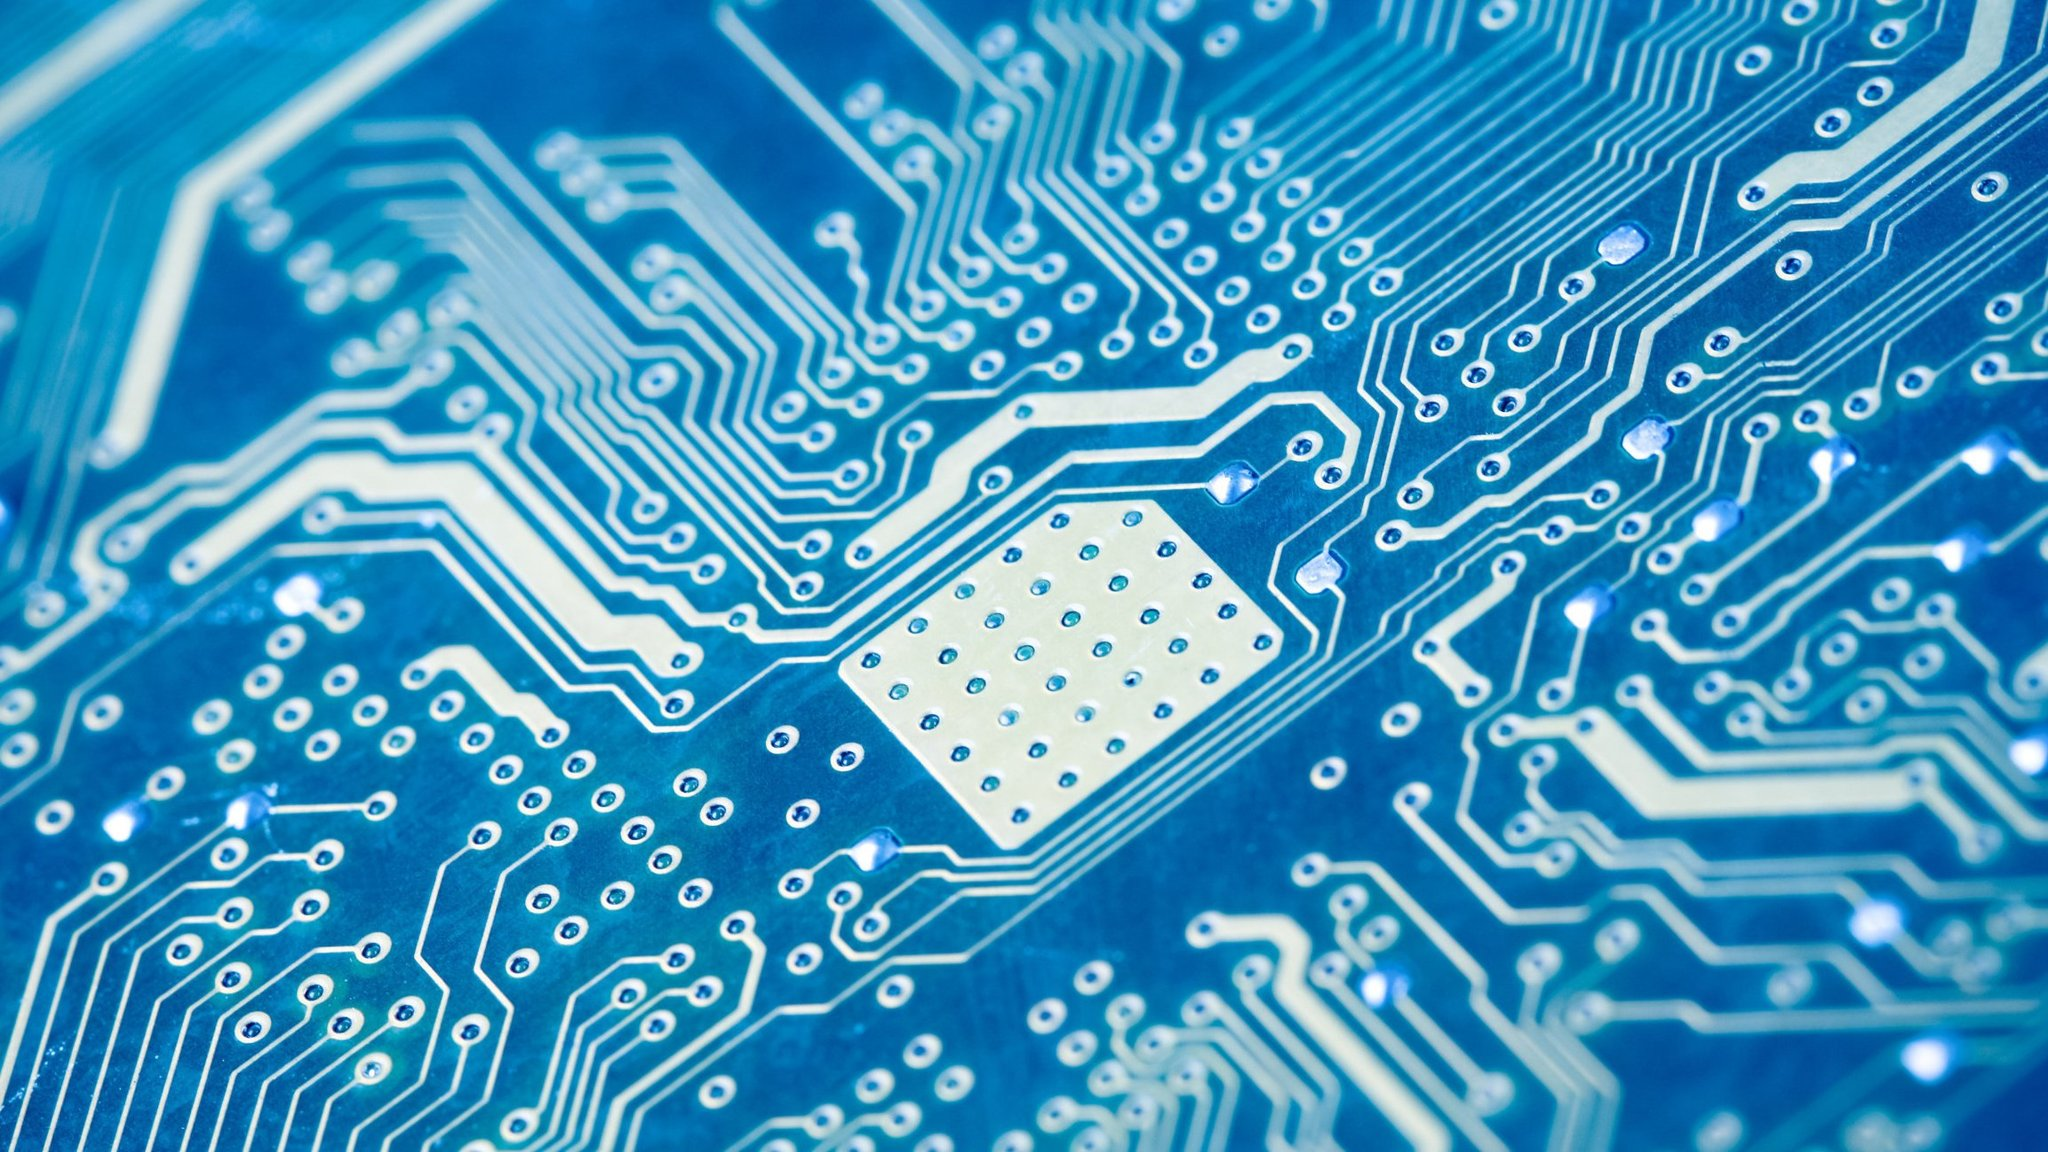
\includegraphics[height=\paperheight,width=\paperwidth]{../03_img/processor.jpg}
			};
		}
		\begin{frame}[plain]
			\vspace*{0.75cm}
			\maketitle
			\vfill
			\begin{center}
				\footnotesize Find all slides on \href{https://github.com/DaWe1992/Applied_ML_Fundamentals}{\linkstyle{GitHub}}
			\end{center}
		\end{frame}
	}
}

% divider page
\newcommand{\makedivider}[1]{
	{
		\beamertemplatenavigationsymbolsempty
		\usebackgroundtemplate{%
			\tikz[overlay,remember picture] \node[opacity=0.2, at=(current page.center)] {
  				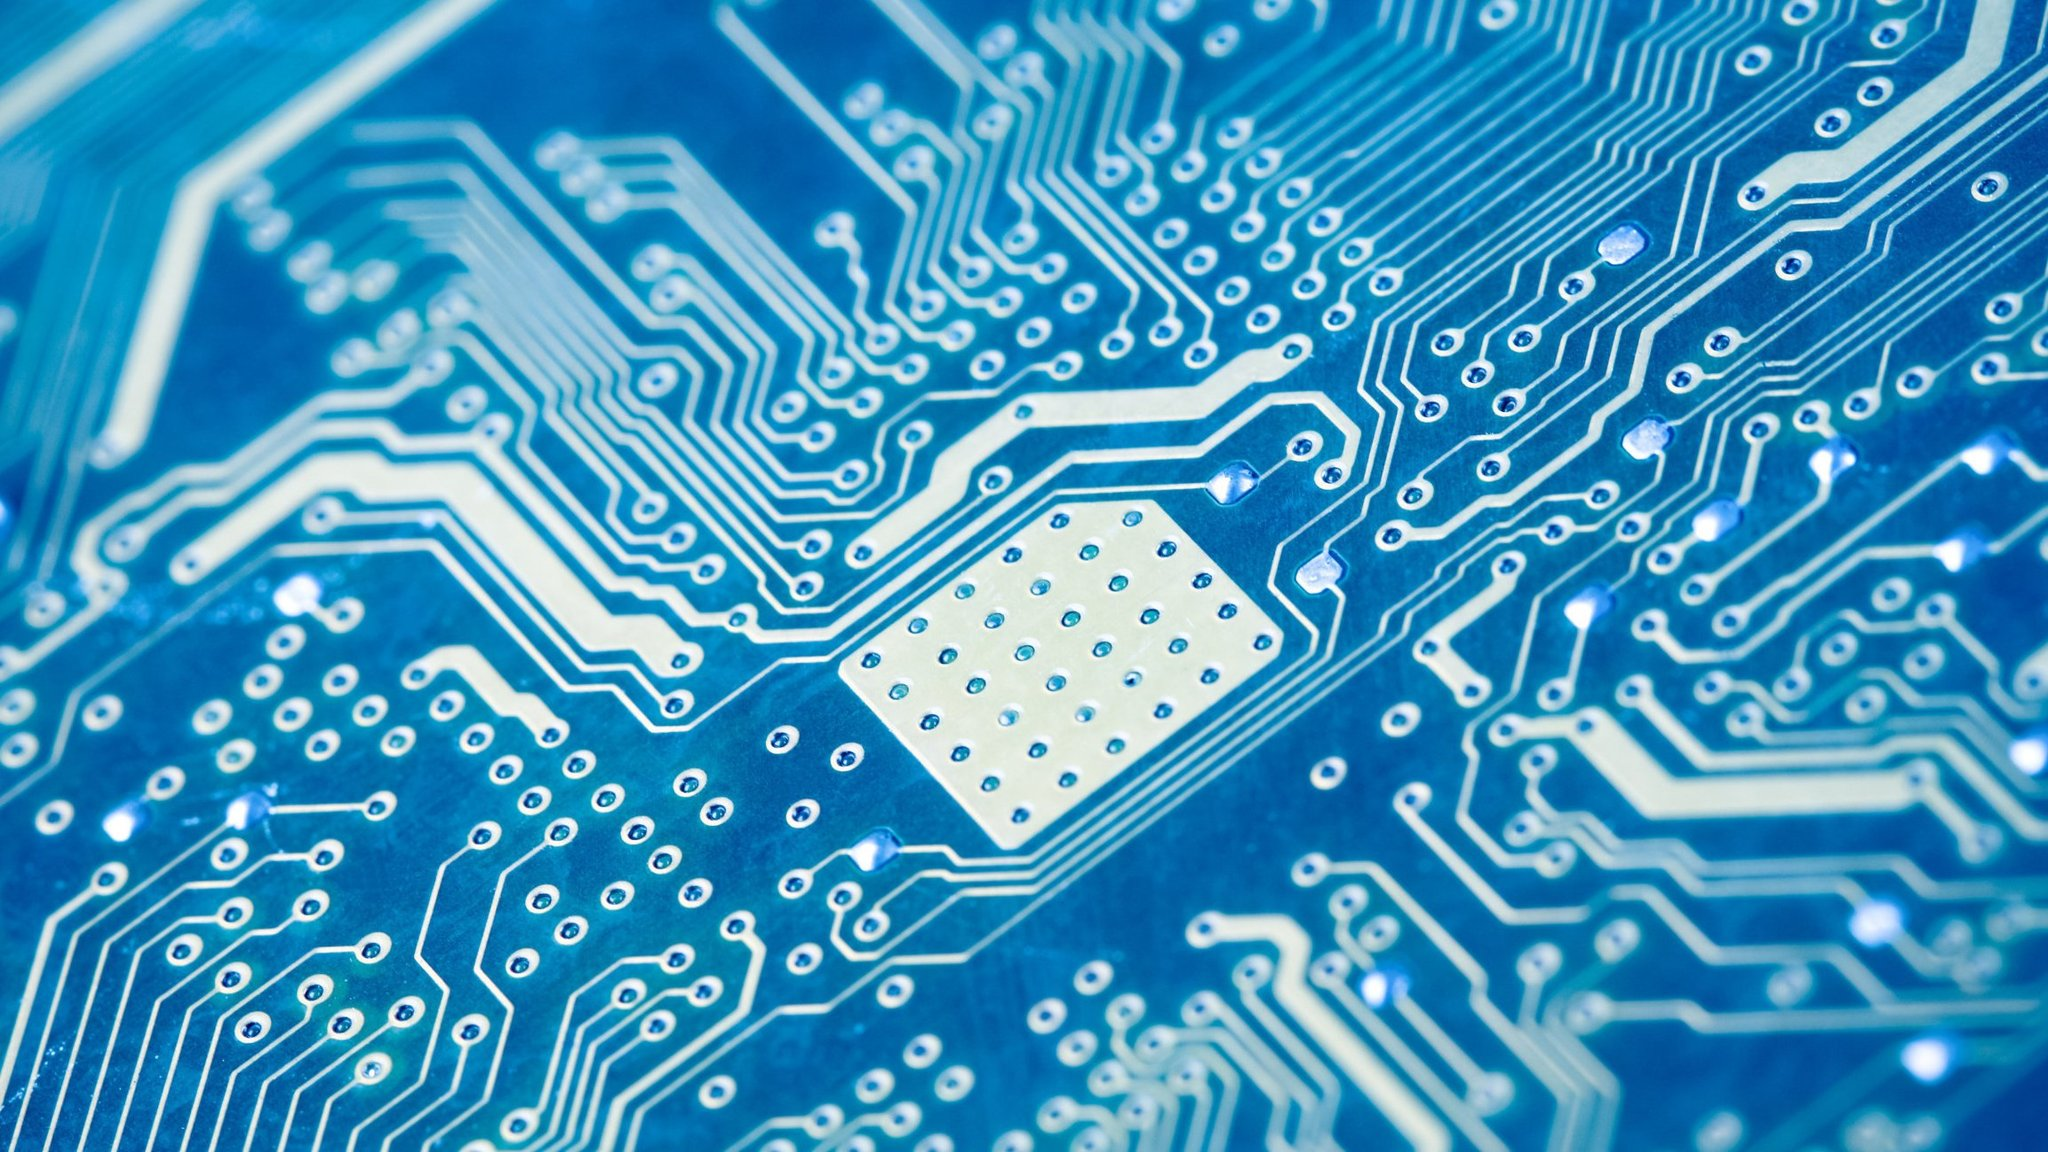
\includegraphics[height=\paperheight,width=\paperwidth]{../03_img/processor.jpg}
			};
		}
		\begin{frame}[plain]
			\vfill
			\begin{boxBlue}
				\centering
				\textbf{Section:} \\
				\large \highlight{#1}
			\end{boxBlue}
			\vfill
			\centering
			
\includegraphics[scale=0.05]{../03_img/logo_dhbw.png}
			\vfill
		\end{frame}
	}
}

% overview page
\newcommand{\makeoverview}[1]{
	\begin{frame}{Lecture Overview}{}
		\begin{tabbing}
			\hspace*{3.5cm}\= \kill
			\ifnum #1=1 \highlight{\textbf{Unit I:}} \else \textbf{Unit I:} \fi
			\> \ifnum #1=1 \highlight{Machine Learning Introduction} \else Machine Learning Introduction \fi \\
		\end{tabbing}
	\end{frame}
}

% thank you page
\newcommand{\makethanks}{
	{\beamertemplatenavigationsymbolsempty
	\begin{frame}[plain]
		\vfill
		\begin{boxBlue}
			\centering
			\Large \highlight{Thank you very much for the attention!}
		\end{boxBlue}
		
		\vfill\footnotesize
		\begin{tabbing}
			\hspace*{1.5cm}\= \kill
			\highlight{Topic:} 	\> \inserttitle \\
			\highlight{Date:} 	\> \insertdate
		\end{tabbing}
		
		\vfill
		\highlight{Contact:} \\
		\insertauthor\ (D062271) \\
		\insertinstitute \\
		\href{mailto:daniel.wehner@sap.com}{\linkstyle{daniel.wehner@sap.com}}
		
		\vfill\normalsize
		\begin{center}
			\large\highlight{Do you have any questions?}
		\end{center}
		\vfill
	\end{frame}}
}

% global pfgplots settings
% --------------------------------------------------------------------------------------------------------
\pgfplotsset{
	% allow filtering of data for pgfplots
	discard if/.style 2 args={
        		x filter/.code={
            		\edef\tempa{\thisrow{#1}}
            		\edef\tempb{#2}
            		\ifx\tempa\tempb
                		\def\pgfmathresult{inf}
            		\fi
        		}
    	},
    	discard if not/.style 2 args={
        		x filter/.code={
            		\edef\tempa{\thisrow{#1}}
            		\edef\tempb{#2}
            		\ifx\tempa\tempb
            		\else
                		\def\pgfmathresult{inf}
            		\fi
        		}
    	}
}


% ====================================================
% ====================================================
% PRESENTATION DATA
% ====================================================
% ====================================================

\title[$k$-Nearest Neighbors]{*** Applied Machine Learning Fundamentals *** $k$-Nearest Neighbors}
\institute{SAP\,SE}
\author{Daniel Wehner}
\date{\today}
\prefix{KNN}

% ====================================================
% ====================================================
% BEGIN OF DOCUMENT
% ====================================================
% ====================================================

\begin{document}

% Title frame
%______________________________________________________________________
\maketitlepage


% Lecture Overview
%______________________________________________________________________
\begin{frame}{Lecture Overview}{}
	\makeoverview{6}
\end{frame}


% Agenda
%______________________________________________________________________
\begin{frame}{Agenda \today}
	\begin{multicols}{2}
		\tableofcontents
	\end{multicols}
\end{frame}


% Section: Introduction
%______________________________________________________________________
\section{Introduction}
\makedivider{Introduction}

% Subsection: Overview of the Algorithm
% --------------------------------------------------------------------------------------------------------
\subsection{Overview of the Algorithm}

% Introduction
\begin{frame}{Introduction}{}
	\divideTwo{0.49}{
		\begin{itemize}
			\item \textbf{Basic idea:} Predict the class label based on nearby known examples
			\item Instance-based learning, a.\,k.\,a. \highlight{lazy learning}
		\end{itemize}
		\vspace*{4mm}
		\begin{boxBlueNoFrame}
			\highlight{We do not learn any model, the data speaks for itself!}
		\end{boxBlueNoFrame}
	}{0.49}{
		\begin{figure}
	\centering
	\begin{tikzpicture}
    
  		  \begin{axis}[
			scale=0.8,
			xlabel={$x_1$},
			ylabel={$x_2$},
			axis x line=center,
  			axis y line=center
		]

			\pgfplotstableread{06_knn/05_data/data_knn_0.txt} \datatableClassZero
			\pgfplotstableread{06_knn/05_data/data_knn_1.txt} \datatableClassOne
		
			\addplot[only marks,mark=*,mark size=2,draw=gray,fill=white] table[x=x,y=y] from \datatableClassZero;
			\addplot[only marks,mark=*,mark size=2,draw=myblue1,fill=white] table[x=x,y=y] from \datatableClassOne;
			\addplot[mark=*,draw=red,fill=red] coordinates {(0.45,0.15)};
		
		\end{axis}
	
		\node[red] at (2.25,0.5) {\textbf{?}};
		
	\end{tikzpicture}
\end{figure}
	}
\end{frame}


% Subsection: Derivation of the Algorithm
% --------------------------------------------------------------------------------------------------------
\subsection{Derivation of the Algorithm}

% Derivation of the Algorithm
\begin{frame}{Derivation of the Algorithm}{}\optional
	\bubble{11}{6}{
		\footnotesize Remember non-parametric \\[-1mm]
		\footnotesize density estimation?
	}
	\begin{itemize}
		\item Unconditional density:
		\begin{equation*}
			p(\bm{x}) = \frac{k}{n \cdot v}
		\end{equation*}
		\item Class priors:
		\begin{equation*}
			p(\mathcal{C}_j) = \frac{n_j}{n}
		\end{equation*}
	\end{itemize}
	
	\begin{boxBlueNoFrame}
		\highlight{Combine using Bayes' theorem:}
		\vspace*{-4mm}
		\begin{equation}
			p(\mathcal{C}_j \vert \bm{x}) 
				= \frac{p(\bm{x} \vert \mathcal{C}_j) \cdot p(\mathcal{C}_j)}{p(\bm{x})}
				= \frac{\frac{k_j}{n_j \cdot v} \cdot \frac{n_j}{n}}{\frac{k}{n \cdot v}}
				= \frac{k_j}{k}
		\end{equation}
	\end{boxBlueNoFrame}
\end{frame}


% Section: Distance Metrics
%______________________________________________________________________
\section{Distance Metrics}
\makedivider{Distance Metrics}

% Subsection: Properties of Distance Metrics
% --------------------------------------------------------------------------------------------------------
\subsection{Properties of Distance Metrics}

% Distance Metrics
\begin{frame}{Distance Metrics}{}
	\begin{itemize}
		\item How to measure the distance between two data points $i$ and $j$? \\
			$\Rightarrow$ \highlight{distance metrics}
		\item Let $d$ be a function $d : (u, v) \mapsto \mathbb{R}^{+}$ (including 0)
		\item Function $d$ has the following properties:
	\end{itemize}
	
	\begin{boxBlueNoFrame}
		\begin{enumerate}
			\item $d(u, v) = d(v, u)$ \highlight{(commutativity)}
			\item $d(u, v) = 0 \Rightarrow u = v$
			\item $d(u, k) \le d(u, v) + d(v, k)$ \highlight{(triangle inequality)}
		\end{enumerate}
	\end{boxBlueNoFrame}
\end{frame}


% Subsection: Minkowski, Manhattan, Euclidean
% --------------------------------------------------------------------------------------------------------
\subsection{Minkowski, Manhattan, Euclidean}

% Distance Metrics (Ctd.)
\begin{frame}{Distance Metrics (Ctd.)}{}
	\highlight{Minkowski distance:}
	\begin{equation}
		d_p(u, v) = \left( \sum_{j=1}^m \vert x_j^{(u)} - x_j^{(v)} \vert \right)^{\nicefrac{1}{p}}
	\end{equation}
	
	\divideTwo{0.49}{
		\highlight{Manhattan distance:} ($p = 1$)
		\begin{equation*}
			d_1(u, v) = \sum_{j=1}^m \vert x_j^{(u)} - x_j^{(v)} \vert
		\end{equation*}
	}{0.49}{
		\highlight{Euclidean distance:} ($p = 2$)
		\begin{equation*}
			d_2(u, v) = \sqrt{\sum_{j=1}^m \vert x_j^{(u)} - x_j^{(v)} \vert^2}
		\end{equation*}
	}
\end{frame}


% Distance Metrics (Ctd.)
\begin{frame}{Distance Metrics (Ctd.)}{}
	\begin{figure}
	\centering
	\begin{tikzpicture}[
		scale=0.9,
		axis/.style={
			->,thick
		},
		point/.style={
			circle,draw=black,
			fill=black,inner sep=2pt
		}
	]
	
		% draw grid
		\draw[lightgray] (0,0) grid (10,5);
		% draw axes
		\draw[axis] (0,0) -- (0,5) node[above]{$x_2$}; \draw[axis] (0,0) -- (10,0) node[right]{$x_1$};
		% axis labels
		\foreach \x in {0,1,...,10} \node at (\x,-0.5){\footnotesize{\x}};
		\foreach \y in {0,1,...,5} \node at (-0.5,\y){\footnotesize{\y}};

		\node[point] (i) at (4,2){};
		\node[point] (j) at (7,4){};

		\draw[red,thick] (i) -- node[above,rotate=32.5,red]{\footnotesize{\textbf{Euclidean}}} (j);
		\draw[blue,thick] (i) -- node[below,blue]{\footnotesize{\textbf{Manhattan}}} ++(3,0) -- (j);

		\node[red,fill=red!30] at (5,5){\footnotesize $d_2(u, v) = \sqrt{(7 - 4)^2 + (4 - 2)^2} = \bm{\sqrt{13}}$};
		\node[blue,fill=myblue1!50] at (5.5,0.75){\footnotesize $d_1(u, v) = |7 - 4| + |4 - 2| = \bm{5}$};

	\end{tikzpicture}
\end{figure}
\end{frame}


% Subsection: Cosine Similarity
% --------------------------------------------------------------------------------------------------------
\subsection{Cosine Similarity}

% Cosine Similarity
\begin{frame}{Cosine Similarity}{}
	\begin{itemize}
		\item \highlight{Similarity metrics} are an alternative to distance metrics
		\item \textbf{Example:} \highlight{Cosine similarity}
		\item The cosine similarity of two vectors $\bm{a}$ and $\bm{b}$ is the cosine of the angle:
		\begin{equation}
			\cos \measuredangle (\bm{a}, \bm{b}) = \frac{\bm{a} \cdot \bm{b}}{\Vert \bm{a} \Vert \cdot \Vert \bm{b} \Vert}
				= \frac{\sum_{j=1}^m a_j \cdot b_j}{\sqrt{\sum_{j=1}^m (a_j)^2} \cdot \sqrt{\sum_{j=1}^m (b_j)^2}}
		\end{equation}
		\item The dot product is defined as:
		\begin{equation}
			\bm{a} \cdot \bm{b} = \Vert \bm{a} \Vert \cdot \Vert \bm{b} \Vert \cdot \cos \measuredangle (\bm{a}, \bm{b})
		\end{equation}
	\end{itemize}
\end{frame}


% Cosine Similarity (Ctd.)
\begin{frame}{Cosine Similarity (Ctd.)}{}
	\begin{figure}
	\centering
	\begin{tikzpicture}[
		scale=0.95
	]

		\fill[lightgray,opacity=0.5] (0,0) -- (4,0) arc[radius=4,start angle=0,end angle=90] -- cycle;
		\draw[gray] (0,0) grid (8,5);
		\draw[thick] (0,4) -- (4,4) -- (4,0);

		\draw[very thick] (0:4) arc[radius=4,start angle=0,end angle=90];

		\fill[gray!70] (0,0) -- (37:2) arc[radius=2,start angle=37,end angle=50] -- cycle;
		\fill[gray] (0,0) -- (50:3) arc[radius=3,start angle=50,end angle=81] -- cycle;

		\draw (37:2) arc[radius=2,start angle=37,end angle=50];
		\draw (50:3) arc[radius=3,start angle=50,end angle=81];
	
		\draw[->,blue,very thick] (0,0) -- (50:3.9);
		\path (0,0) -- (50:4) node[circle,draw=black,fill=blue,inner sep=0.2em] {};
		\draw[->,red,very thick] (0,0) -- (37:3.9);
		\path (0,0) -- (37:4) node[circle,draw=black,fill=red,inner sep=0.2em] {};
		\draw[->,orange,very thick] (0,0) -- (81:3.9);
		\path (0,0) -- (81:4) node[circle,draw=black,fill=orange,inner sep=0.2em] {};

		\node at (1.325,1.25) {\footnotesize{$\alpha_1$}};
		\node at (1,2) {\footnotesize{$\alpha_2$}};

		\node at (2.8,3.5) {$\bm{u}$};
		\node at (3.75,2.5) {$\bm{v}_1$};
		\node at (0.75,4.5) {$\bm{v}_2$};

		\node at (4,-0.5) {1};
		\node at (-0.5,4) {1};

		\node[align=left,black,rectangle,draw=black,fill=lightgray] at (8,2.5) {
			$\bm{v}_1$ is closer to $\bm{u}$, \\
			since \\
			$\cos(\alpha_1) < \cos(\alpha_2)$ \\
			--------------------------- \\
			$\cos(0) = 1$ \\
			$\cos(90) = 0$
		};

		\draw[->,thick] (0,0) -- (8,0) node[right] {$x_1$};
		\draw[->,thick] (0,0) -- (0,5) node[above] {$x_2$};

	\end{tikzpicture}
\end{figure}
\end{frame}


% Section: $k$-nearest Neighbors Algorithm
%______________________________________________________________________
\section{$k$-nearest Neighbors Algorithm}
\makedivider{$k$-nearest Neighbors Algorithm}

% Subsection: General Procedure
% --------------------------------------------------------------------------------------------------------
\subsection{General Procedure}

% Prediction with $k$-Nearest Neighbors (Ctd.)
\begin{frame}{Prediction with $k$-Nearest Neighbors (Ctd.)}{}
	\highlight{$k$-nearest neighbors algorithm:}
	\begin{enumerate}
		\item Calculate the distances between the new data point and \textbf{all data points in the data set}
		\item Sort the data points by distances \textbf{in ascending order} \\
			{\footnotesize \textit{(if similarity metrics are used, sort in descending order)}}
		\item Look at the first $k$ examples and \textbf{count how often each class occurs}
		\item Predict the class with \textbf{the maximum score}
	\end{enumerate}
\end{frame}


% Subsection: Calculation of Distances
% --------------------------------------------------------------------------------------------------------
\subsection{Calculation of Distances}

% \ding{182} Calculation of Distances
\begin{frame}{\ding{182} Calculation of Distances}{}
	\divideTwo{0.49}{
		\vspace*{3mm}
		\begin{table}
	\scalebox{0.7}{
	\begin{tabular}{| c | c | c | c | c |}
		\hline
		\rowcolor{lightgray}
		$v$			&
		$x_1$ 		&
		$x_2$ 		&
		$\mathcal{C}$ 	&
		$d_2(u, v)$ 	\\
		\hline\hline
		1 			& 0.66 		& 0.24 		& 1 			& 0.23		\\ \hline
		2 			& 0.25 		& 0.79 		& 1 			& 0.67		\\ \hline
		3 			& 0.16		& 0.81		& 1 			& 0.73		\\ \hline
		4 			& 0.57		& 0.21		& 1 			& 0.13		\\ \hline
		5 			& 0.21		& 0.72		& 1 			& 0.62		\\ \hline
		6 			& 0.66		& 0.27		& 1 			& 0.24		\\ \hline
		7 			& 0.27		& 0.11		& 0 			& 0.19		\\ \hline
		8 			& 0.39		& 0.13		& 0 			& 0.07		\\ \hline
		9 			& 0.39		& 0.86		& 0 			& 0.71		\\ \hline
		10 			& 0.44		& 0.67		& 0 			& 0.52		\\ \hline
		11 			& 0.31		& 0.33		& 0 			& 0.23		\\ \hline
		12			& 0.03		& 0.51		& 0 			& 0.55		\\ \hline
		$\vdots$		& $\vdots$	& $\vdots$	& $\vdots$	& $\vdots$ 	\\ \hline
	\end{tabular}}
\end{table}
	}{0.49}{
		\begin{itemize}
			\item $\bm{x}^{(u)} = (0.45, 0.15)$
			\item Calculate the \textbf{Euclidean distance} between $\bm{x}^{(u)}$ and all other data points $\bm{x}^{(v)}$
		\end{itemize}
		\vspace*{3mm}
		\begin{boxBlueNoFrame}
			\highlight{Prediction is expensive!}
		\end{boxBlueNoFrame}
	}
\end{frame}


% Subsection: Prediction of the Class Label
% --------------------------------------------------------------------------------------------------------
\subsection{Prediction of the Class Label}

% \ding{183}/\ding{184}/\ding{185} Prediction of the Class Label
\begin{frame}{\ding{183}/\ding{184}/\ding{185} Prediction of the Class Label}{}
	\divideTwo{0.49}{
		\begin{itemize}
			\item Let $k$ be set to 10
			\item Step \ding{183}: Sort data set by distances \\
				{\footnotesize \textit{(cf. table)}}
			\item Step \ding{184}: Count the classes
			\begin{itemize}
				\item \textbf{Class 0:} 3
				\item \textbf{Class 1:} 7
			\end{itemize}
			\item Step \ding{185}: \textbf{Predict class 1!}
		\end{itemize}
	}{0.49}{
		\vspace*{3mm}
		\begin{table}
	\scalebox{0.75}{
	\begin{tabular}{| c | c | c | c |}
		\hline
		\rowcolor{lightgray}
		$x_1$ 			&
		$x_2$ 			&
		$\mathcal{C}$ 		&
		$d_2(u, v)$ 		\\
		\hline\hline
		0.51 		& 0.17 		& 1 			& 0.06		\\ \hline
		0.39 		& 0.13 		& 0 			& 0.07		\\ \hline
		0.52 		& 0.17 		& 1 			& 0.08		\\ \hline
		0.43 		& 0.23 		& 0 			& 0.08		\\ \hline
		0.47 		& 0.03 		& 0 			& 0.12		\\ \hline
		0.52 		& 0.26 		& 1			& 0.13		\\ \hline
		0.57 		& 0.21 		& 1 			& 0.13		\\ \hline
		0.53 		& 0.25 		& 1 			& 0.13		\\ \hline
		0.58 		& 0.12	 	& 1 			& 0.14		\\ \hline
		0.59 		& 0.13 		& 1 			& 0.14		\\ \hline
		$\vdots$	& $\vdots$	& $\vdots$	& $\vdots$	\\ \hline
	\end{tabular}}
\end{table}
	}
\end{frame}


% Section: Choice of $k$
%______________________________________________________________________
\section{Choice of $k$}
\makedivider{Choice of $k$}

% Subsection: Danger of Overfitting
% --------------------------------------------------------------------------------------------------------
\subsection{Danger of Overfitting}

% How to choose $k$
\begin{frame}{How to choose $k$?}{}
	\textbf{The choice of $k$ is important:} \\
	\divideTwo{0.49}{
		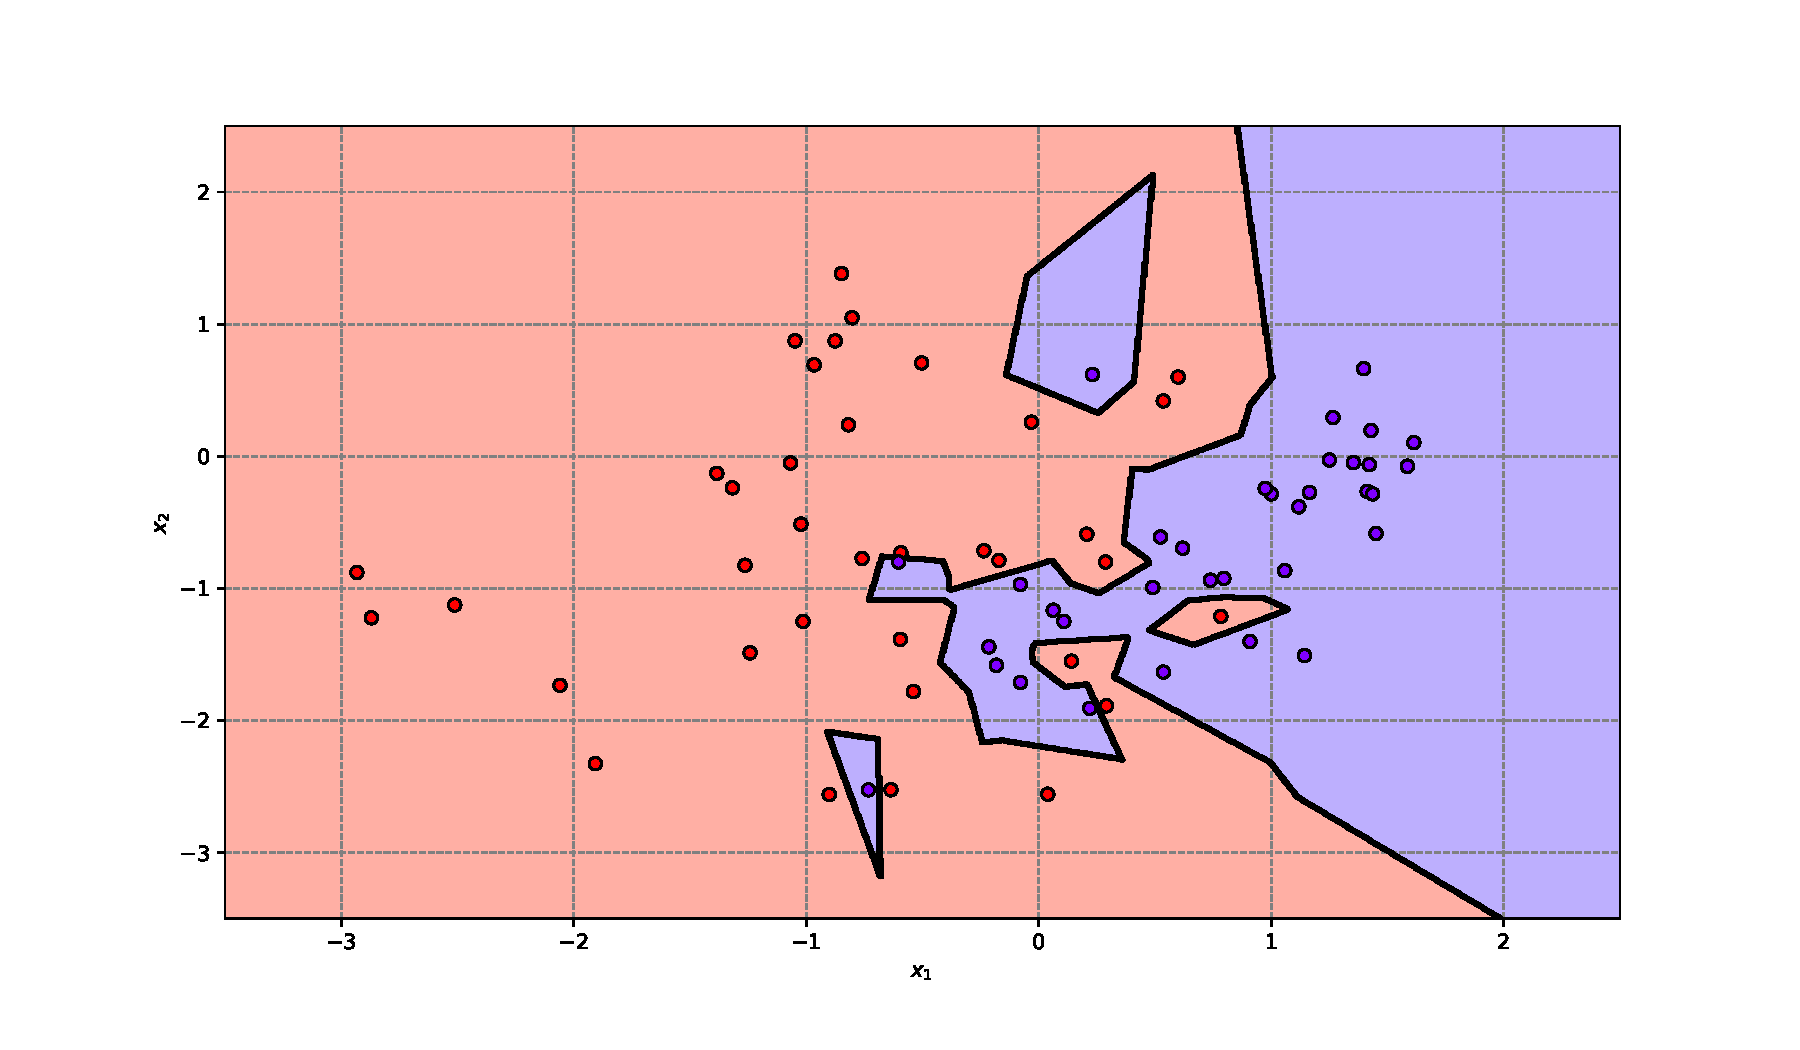
\includegraphics[scale=0.25]{06_knn/02_img/knn_1}
		\vspace*{-3mm}
		\begin{center}
			\hspace*{7mm}
			$k = 1$ \Highlight{($\skull$ overfitting $\skull$)}
		\end{center}
	}{0.49}{
		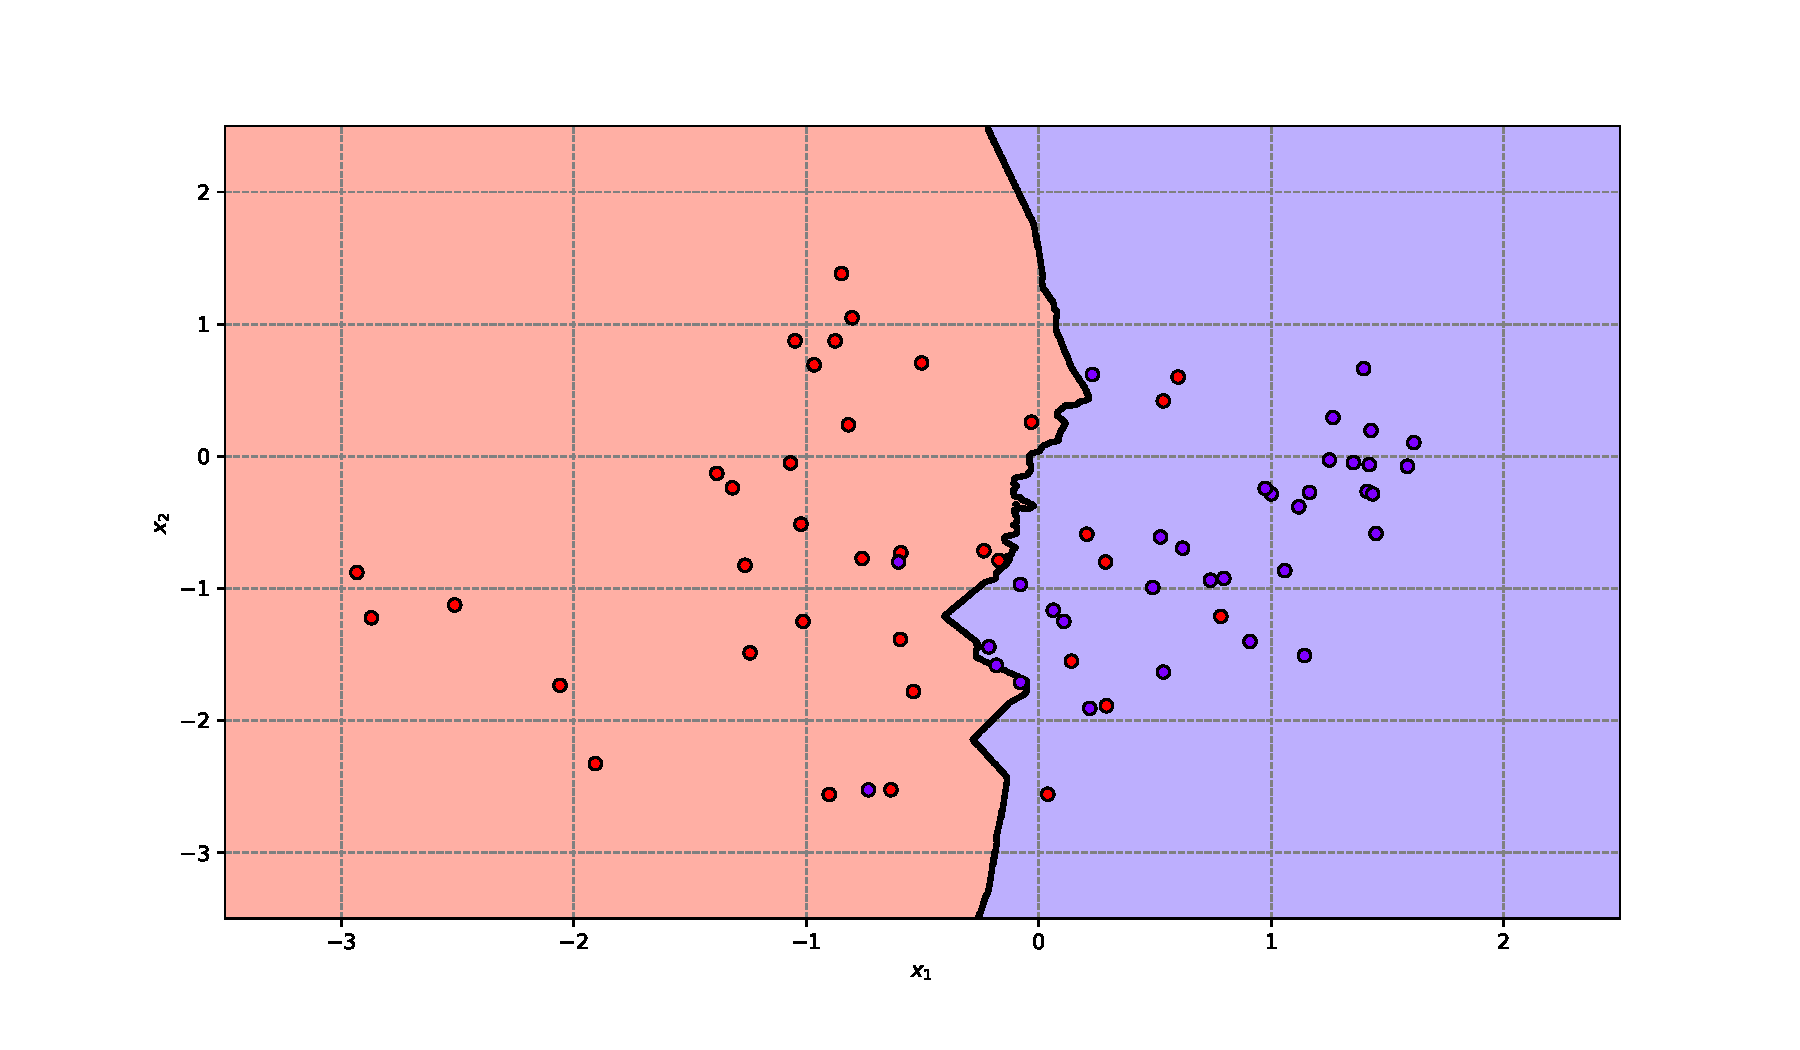
\includegraphics[scale=0.25]{06_knn/02_img/knn_30}
		\vspace*{-3mm}
		\begin{center}
			\hspace*{7mm}
			$k = 30$ (about right)
		\end{center}
	}
\end{frame}


% Subsection: Selection Strategies
% --------------------------------------------------------------------------------------------------------
\subsection{Selection Strategies}

% How to choose $k$ (Ctd.)
\begin{frame}{How to choose $k$? (Ctd.)}{}
	\begin{itemize}
		\item First of all, it is recommended to use \textbf{odd values} for $k$ \\
			{\footnotesize \textit{(no tie-breaking necessary)}}
		\item Compute $k$ depending on the size of the data set $\mathcal{D}$:
		\begin{equation}
			k = \sqrt{\frac{n}{2}} \qquad \text{or} \qquad k = \sqrt{n}
		\end{equation}
		\item \textbf{Other strategy:} Evaluate different $k$ on a \texttt{dev} set and choose the best one
	\end{itemize}
\end{frame}


% How to choose $k$ (Ctd.)
\begin{frame}{How to choose $k$? (Ctd.)}{}
	\begin{figure}
	\centering
	\begin{tikzpicture}[
		scale=1.0
	]

		\begin{axis}[
			grid=both,
    			grid style={line width=0.1pt, draw=lightgray!70},
			xlabel={$k$},
			ylabel={Error},
			y=0.28cm,
    			x=0.2cm,
			ymax=20
		]
    			\pgfplotstableread{06_knn/05_data/data_choose_k.txt} \datatable
			\addplot[mark=*,mark size=1.5,myblue1] table[x=x,y=y] from \datatable;

			\node[gray] (A) at (axis cs:10,15) {\textbf{best} $k$: 8 or 9};
			\draw[->,thick,gray] (A) -- (axis cs:8.5,6.5);
			\draw[gray,very thick] (axis cs:7,5.7) -- (axis cs:10,5.7);
			
    		\end{axis}

	\end{tikzpicture}
\end{figure}
\end{frame}


% Section: Wrap-Up
%______________________________________________________________________
\section{Wrap-Up}
\makedivider{Wrap-Up}

% Subsection: Summary
% --------------------------------------------------------------------------------------------------------
\subsection{Summary}

% Summary
\begin{frame}{Summary}{}
	\begin{itemize}
		\item The basic idea is to classify unknown instances \textbf{based on nearby examples}
		\item The algorithm is an example for \textbf{instance-based learning}
		\item \textbf{Distance metrics} allow to calculate the distance between data points:
		\begin{itemize}
			\item Manhattan distance
			\item Euclidean distance
			\item Cosine similarity
		\end{itemize}
		\item Choose the value of $k$ wisely:
		\begin{itemize}
			\item Too small: \textbf{Overfitting}
			\item Too large: \textbf{Underfitting}
		\end{itemize}
	\end{itemize}
\end{frame}


% Subsection: Self-Test Questions
% --------------------------------------------------------------------------------------------------------
\subsection{Self-Test Questions}

% Self-Test Questions
\begin{frame}{Self-Test Questions}{}\important
	\begin{enumerate}
		\item Outline the $k$-nearest neighbors algorithm.
		\item What is instance-based learning (in contrast to model-based learning)?
		\item How can you compute distances? What properties do distance metrics have?
		\item What is the intuition behind the triangle inequality?
		\item How can you choose $k$?
		\item Suppose you have a data set comprising $n = 50$ examples. \\
			If you set $k = n$, what class does the algorithm predict?
		\item What are advantages and disadvantages of the algorithm?
	\end{enumerate}
\end{frame}


% Subsection: Lecture Outlook
% --------------------------------------------------------------------------------------------------------
\subsection{Lecture Outlook}

\begin{frame}{What's next...?}{}
	\makeoverview{6}
\end{frame}


% Subsection: Recommended Literature and further Reading
% --------------------------------------------------------------------------------------------------------
\subsection{Recommended Literature and further Reading}

% Literature
%______________________________________________________________________
\begin{frame}{Recommended Literature and further Reading}{}
	\footnotesize
	\begin{thebibliography}{2}

	\end{thebibliography}
\end{frame}


% Subsection: Meme of the Day
% --------------------------------------------------------------------------------------------------------
\subsection{Meme of the Day}

% Meme of the Day
\begin{frame}{Meme of the Day}{}
	\begin{figure}
		
\includegraphics[scale=0.225]{06_knn/02_img/meme_of_the_day}
	\end{figure}
\end{frame}


% Thank you
%______________________________________________________________________
\makethanks

\end{document}